\chapter{Dados Reais} \label{cap:dadosreais}
\vspace{-2cm}

Durante o período de maio a julho de 2017 foram feitas aquisições de dados do detector para raios cósmicos, utilizando duas pás cintiladoras de dimensões $14$x$14$x$1$ posicionadas acima do plano superior do detector como sistema de \emph{trigger}. A primeira pá foi posicionada a $4.5$ cm acima da superfície superior do detector enquanto a segunda pá foi posicionada a $47.5$ cm da mesma superfície.

O sistema de \emph{trigger} foi configurado para realizar a aquisição dos dados das PMTs caso ambas as pás cintiladoras tenham detectado um sinal, fazendo a aquisição dos dados salvos nos \emph{buffers} das NDAQs, salvando as últimas $100$ amostras digitalizadas. Foram selecionados no total $9999$ eventos consecutivos registrados pelo detector para análise deste trabalho.



\section{Metodologia de análise dos dados do experimento}

Os dados do experimento são salvos em arquivos de texto com o valor analógico da saída de cada PMT convertido para um valor digital, valor tal será referido como \emph{ADC counts} a partir deste ponto. Podemos estimar a quantidade de p.e. total por evento estimando a contagem de  \emph{ADC counts} no pico do mesmo, assim, a estratégia para a análise será estimar a quantidade de p.e. por PMT por evento, verificar a quantidade de p.e. por evento e por PMT.

Como no sistema existe uma tensão de \emph{bias} negativa, conhecida como pedestal, precisamos removê-la antes de começar uma análise mais profunda dos dados, centralizando nossas amostras no valor nulo. O pedestal pode ser visto e comparado com uma amostra sem o mesmo na Figura \ref{fig:pedestal}.

\begin{figure}[H]
	\centering
	%	\hspace*{-2cm}
	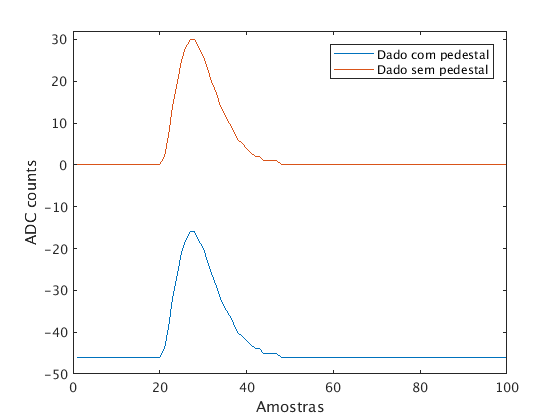
\includegraphics[width=14cm]{textuais/dadosreais/figuras/pedestal.png}
	\caption{Sinal com e sem pedestal}
	\label{fig:pedestal}
\end{figure}

Afim de definir o número de p.e. de cada PMT verificamos o valor máximo de cada PMT. Devido à saturação das PMTs e da eletrônica de \emph{front-end}, os dados coletados com pico de energia acima do valor de saturação devem ser recuperados de alguma forma, foi utilizado um \emph{fitting} com uma forma do sinal conhecida através de um processo iterativo, calculando o erro provável de uma área linear pelo teste do $\chi^2$ (qui-quadrado, Apêndice \ref{apdx:qui-quadrado}) e utilizando a forma final com menor erro, estimando assim, a forma do sinal não saturado. Um exemplo de sinal saturado e sua estimação está presente na FIgura \ref{fig:saturado}.

\begin{figure}[H]
	\centering
%	\hspace*{-2cm}
	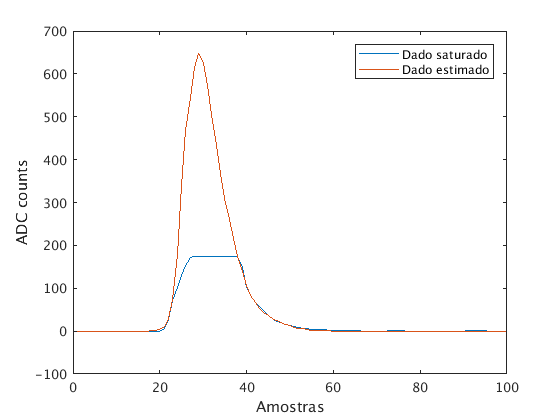
\includegraphics[width=14cm]{textuais/dadosreais/figuras/saturado.png}
	\caption{Sinal de uma PMT saturada versus sua estimação de pico}
	\label{fig:saturado}
\end{figure}

Para verificar as quantidades de p.e. por evento e por PMT, será feito um histograma para cada caso. 

\section{Debug dos dados reais}


Após o \emph{fit} dos dados, foi encontrado um problema intrínseco ao método, como o \emph{fit} era realizado a partir do ponto de saturação eventos naquele ponto foram, em sua maioria, removidos do sistema como pode ser visto no histograma da Figura \ref{fig:peakdist_errado}.

Para resolver este problema precisamos modificar o modo de \emph{fit} a ser realizado. Foi feito então o mesmo método anterior, porém a partir de um ponto em que as PMTs não estão em saturação, mantendo o valor próprio e estimando os valores além de do ponto não saturado, resolvendo o erro de estimação e gerando a Figura \ref{fig:peakdist}.

\begin{figure}[H]
	\centering
%	\hspace*{-2cm}
	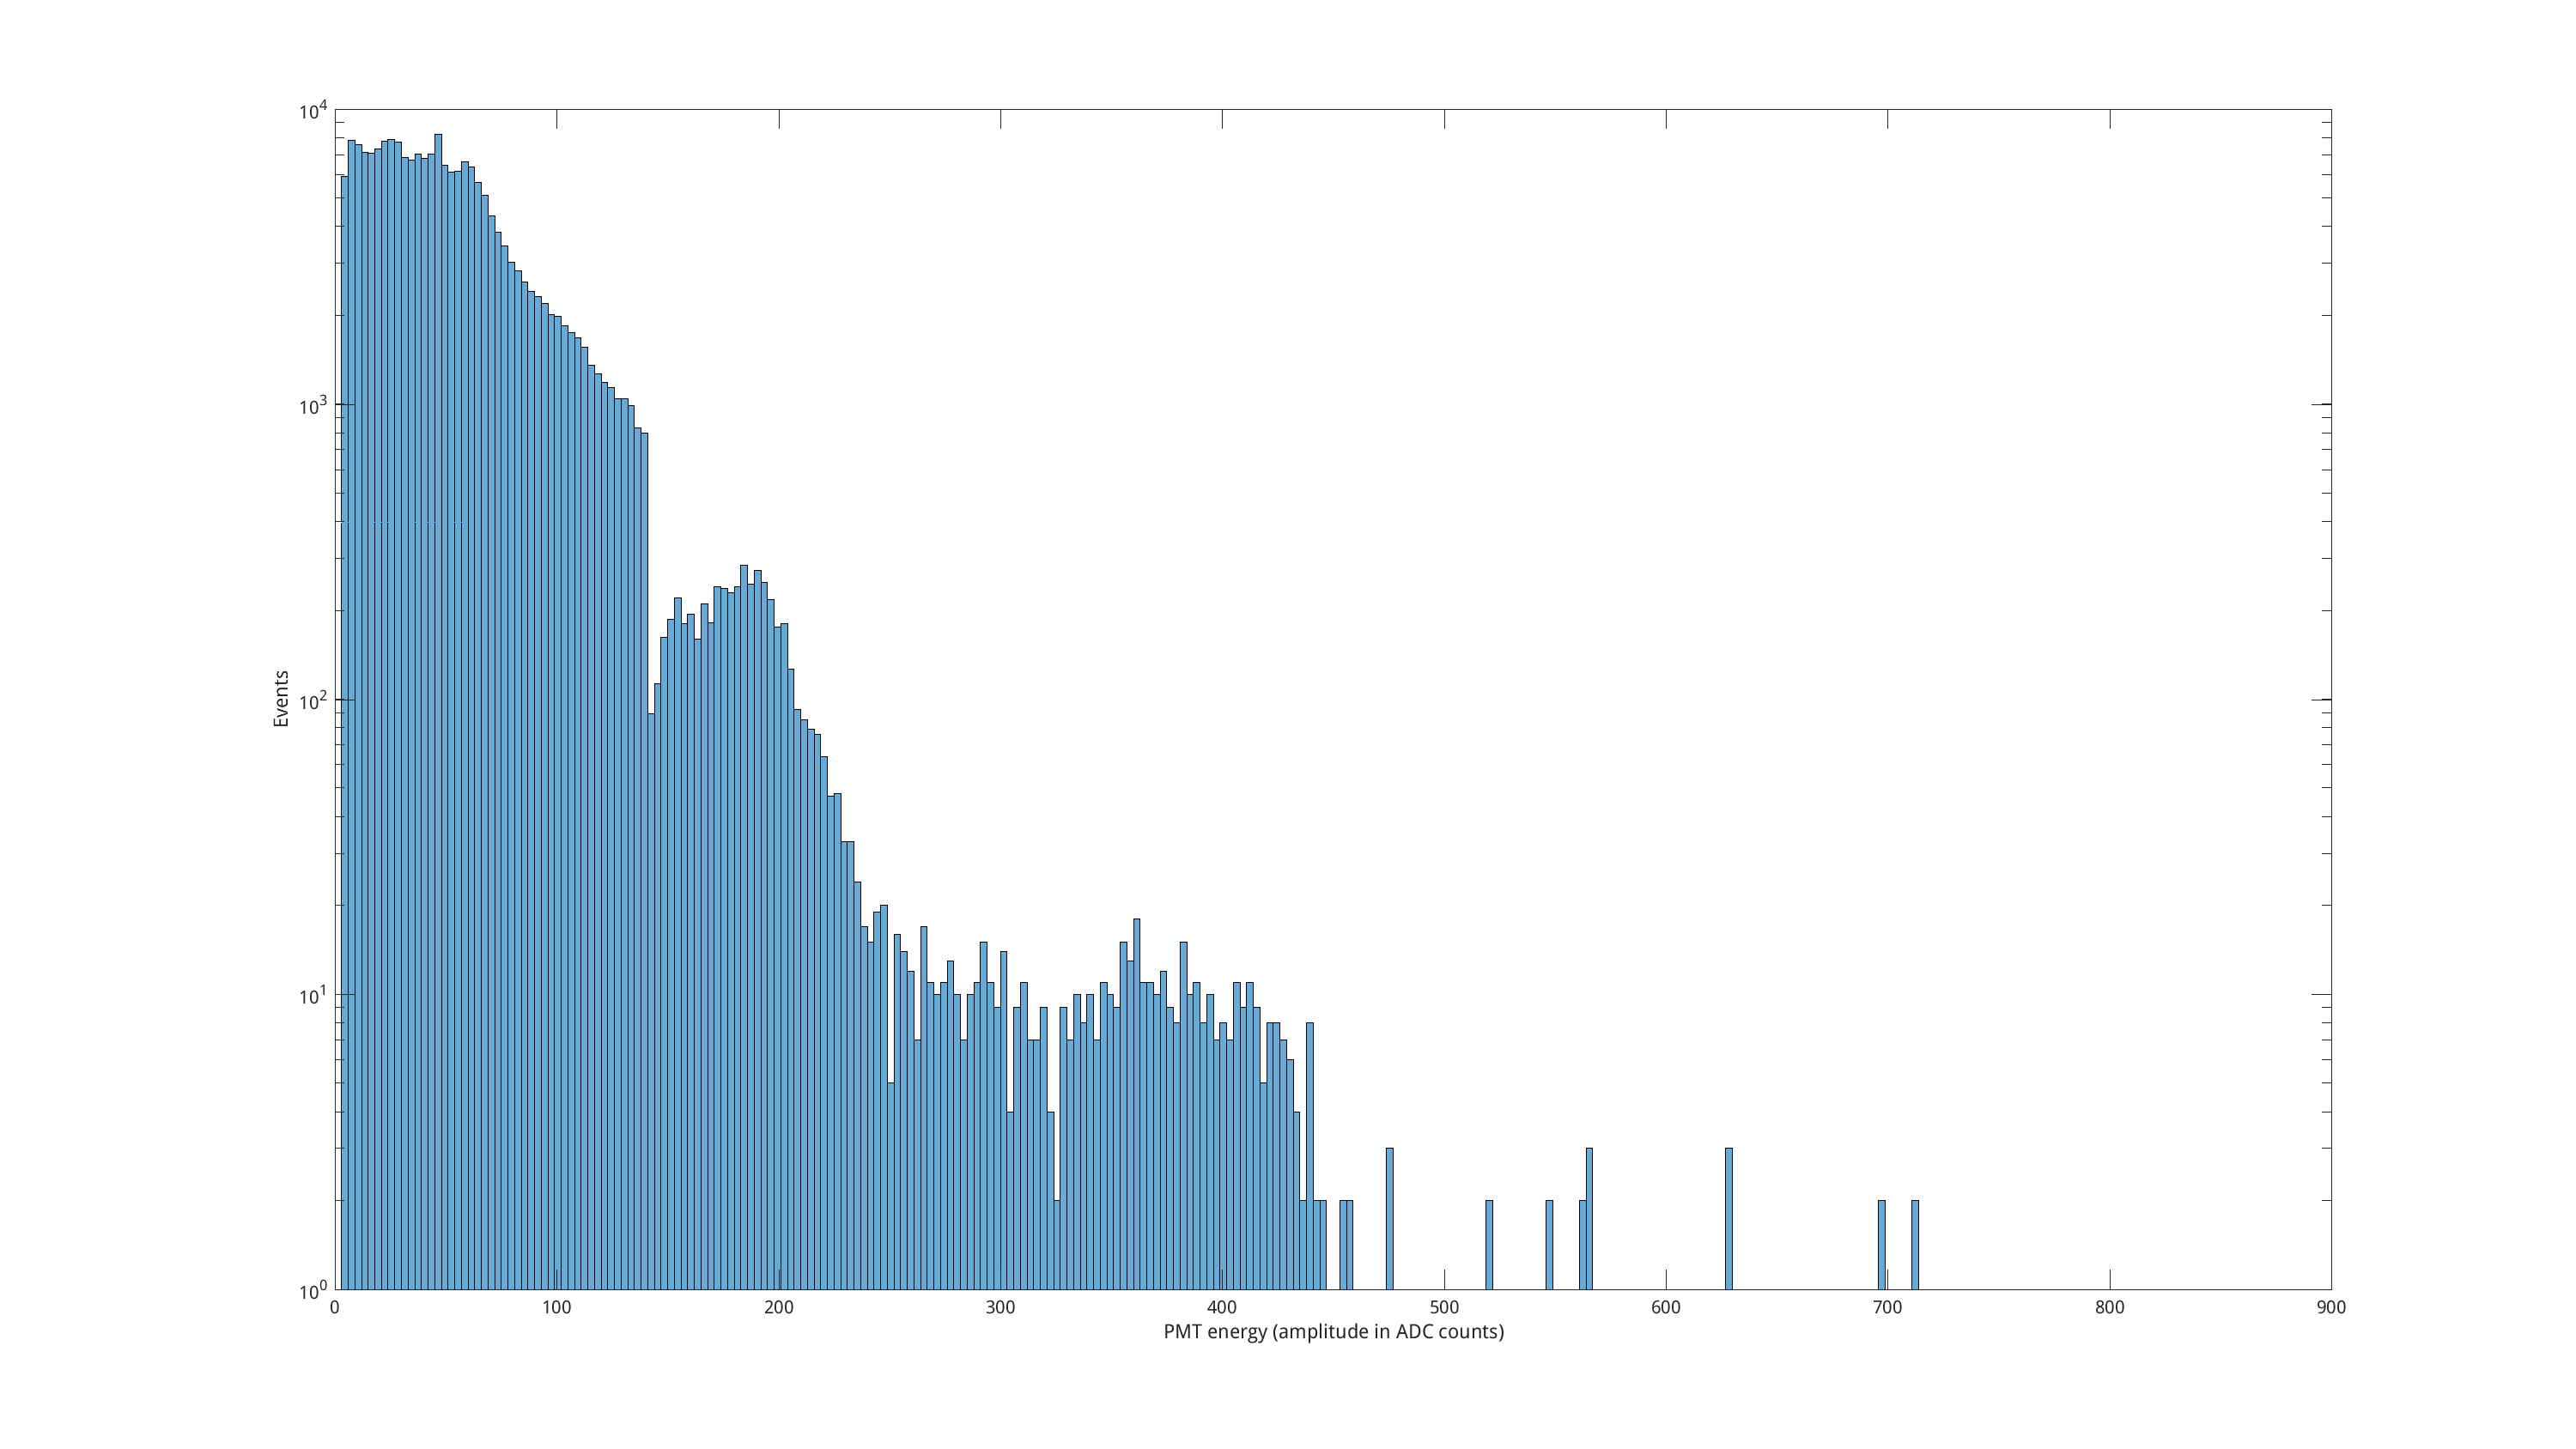
\includegraphics[width=14cm]{textuais/dadosreais/figuras/peakdist_errado.png}
	\caption{Distribuição de picos com problema causado pela estimação}
	\label{fig:peakdist_errado}
\end{figure}

\begin{figure}[H]
	\centering
	%	\hspace*{-2cm}
	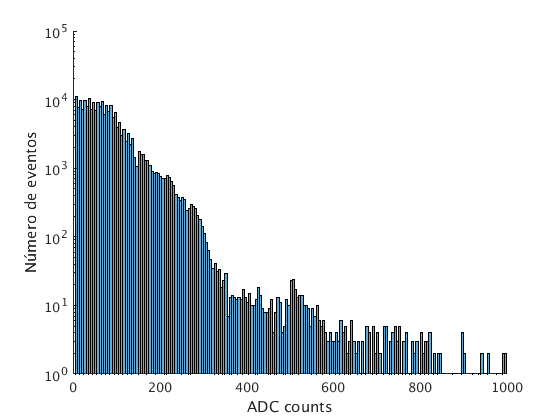
\includegraphics[width=14cm]{textuais/dadosreais/figuras/peakdist.png}
	\caption{Distribuição de picos após a resolução do problema de estimação}
	\label{fig:peakdist}
\end{figure}


\section{Dados da aquisição}

Após resolver os problemas de saturação e estimação dos sinais, temos os dados  a serem comparados com a simulação, representados pelas Figuras \ref{fig:peakdist} e \ref{fig:hist_evt}.

A Figura \ref{fig:hist_evt} representa a quantidade de p.e. por evento, ou seja, a soma de todas as PMTs do detector central, e a Figura \ref{fig:peakdist} representa a distribuição de p.e. para todas as PMTs indivitualmente.
\\

\begin{figure}[H]
	\centering
%	\hspace*{-2cm}
	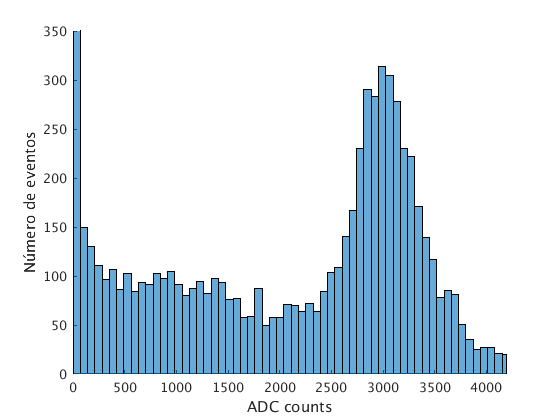
\includegraphics[width=14cm]{textuais/dadosreais/figuras/hist_evt.png}
	\caption{Distribuição de picos após a resolução do problema do \emph{fit}}
	\label{fig:hist_evt}
\end{figure}

